% vim: set textwidth=78 autoindent:

\subsection{Complemento de impresi�n r�pida}

% when the revision of a section has been finalized, 
% comment out the following line:
% \updatedisclaimer

El complemento \toolbtntwo{quick_print}{Impresi�n R�pida} hace posible exportar el canvas del mapa actual a un formato PDF r�pidamente y f�cilmente, con esfuerzo m�nimo. Los �nicos par�metros que necesitan ser especificados son el T�tulo del Mapa, un nombre del mapa y el tama�o del papel (vea la figura ~\ref{fig:quickprint}). 
Si requiere control adicional sobre el dise�o del mapas, 
por favor use el Dise�ador de Impresi�n, descrito en la secci�n~\ref{label_printcomposer}.  

\begin{figure}[ht]
   \begin{center}
   \caption{Di�logo de impresi�n r�pida \nixcaption}\label{fig:quickprint}\smallskip
   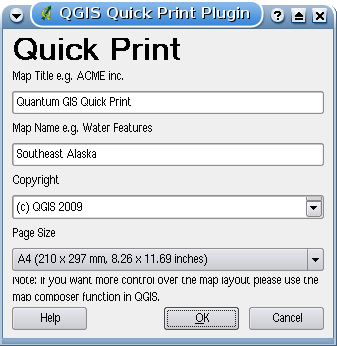
\includegraphics[clip=true, width=6cm]{quick_print_dialog}
\end{center}
\end{figure}

\begin{figure}[ht]
   \begin{center}
   \caption{Resultado de Impresi�n R�pida como DIN A4 PDF usando el conjunto de datos de ejemplo de alaska \nixcaption}\label{fig:quickprint_result}\smallskip
   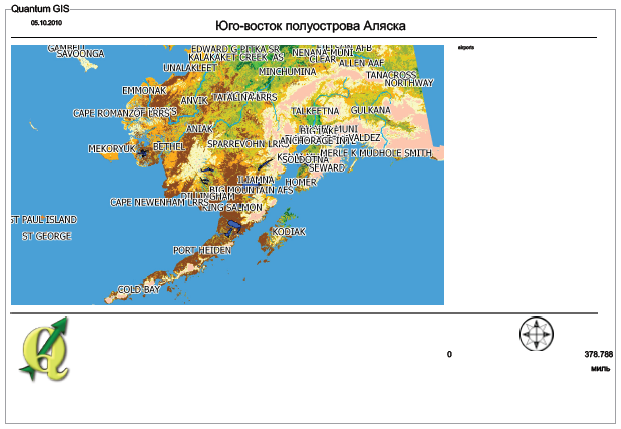
\includegraphics[clip=true, width=9cm]{quick_print_result}
\end{center}
\end{figure}
